\documentclass{article}

\usepackage{amsmath}
\usepackage[utf8]{inputenc}
\usepackage[margin=0.5in]{geometry}
\usepackage{listings}
\usepackage{graphicx}
\usepackage{subcaption}

\lstset{
	columns=fullflexible,
	frame=single,
	breaklines=true,
}

\title{Midterm	2}
\author{Miguel A. Gomez B.}

\begin{document}
	\maketitle
\paragraph{1} List the matrix form of the numerical solver techniques for solving the heat diffusion equation.
\paragraph{Solution}
Given that:
\begin{itemize}
	\item $I$ is the identity matrix.
	\item $A$ is the matrix that contains the generalization of the factors of the linear equations.
	\item $\Delta t$ is the simulation parameter for time.
	\item $a$ is the diffusion coefficient of the material.
	\item $h$ is the simulation parameter for an one-dimensional space rod.
	\item $\overrightarrow{\rm U}_0$ is the initial solution of the ODE.
\end{itemize}
\textbf{The explicit solver:}
$$ \overrightarrow{\rm U}^{n+1} = \left(I + A\frac{\Delta t a}{h^2}\right)^{n+1} \cdot \overrightarrow{\rm U}_0$$
\textbf{The implicit solver:}
$$\overrightarrow{\rm U}^{n+1} = \left(I - A\frac{\Delta t a}{h^2}\right)^{-1} \cdot \overrightarrow{\rm U}_{0}$$
\textbf{The Crank-Nicolson solver:}
$$\overrightarrow{\rm U}^{n+1} = \left[\left(I + A\frac{\Delta t a}{h^2}\right) \cdot \left(I - A \frac{\Delta t a}{h^2}\right)^{-1} \right]^{n+1} \cdot \overrightarrow{\rm U}_{0}$$
\paragraph{2} Write a program to use the explicit method to solve the diffusion equation
\begin{align*}
	u_t &= u_{xx}, t > 0, 0 < x < 1;\\
	u(0, t) &= 0; \\
	u(1, t) &= e^{-\pi^2 \frac{t}{4}}; \\
	u(x, 0) &= \sin{\left(\pi \frac{x}{2}\right)}.
\end{align*}
which has the exact solution:
$$u(x, t) = e^{-\pi^2 \frac{t}{4}} \sin{\left(\pi \frac{x}{2}\right)}$$
(the student should check that this is indeed the exact solution). Use $h^{-1} = 4, 8, \dots, \frac{1}{1024}$, and take $\Delta t$ as large as possible to maintain stability. Confirm that the approximate solution is as accurate as the theory predicts. Compute out to $t = 1$.
\paragraph{Solution} We use the initial solutions and test them on the analytical solution, it is expected to obtain the formulas of the initial solutions:
\begin{align*}
	U(0,t) &= e^{-\pi^2 \frac{t}{4}} \sin{\left(\pi \frac{0}{2}\right)}\\
	&= e^{-\pi^2 \frac{t}{4}}\sin{(0)}\\
	&= 0
\end{align*}
\begin{align*}
	U(1,t) &= e^{-\pi^2 \frac{t}{4}} \sin{\left(\pi \frac{1}{2}\right)}\\
	&= e^{-\pi^2 \frac{t}{4}}\sin{\left(\frac{\pi}{2}\right)}\\
	&= e^{-\pi^2 \frac{t}{4}}
\end{align*}
\begin{align*}
U(x,0) &= e^{-\pi^2 \frac{0}{4}} \sin{\left(\pi \frac{x}{2}\right)}\\
&= \sin{\left(\pi\frac{x}{2}\right)}\\
\end{align*}
We conclude that the analytical solution is correct. Next, to solve this problem we'll use the Explicit method solver with a modification to test each $h$ to explore which would be the best solution. Notice that the condition $0 < x < 1$ implies that we must use exclusively $\sin{\left(\pi \frac{x}{2}\right)}$ as the generator of the main approximation function.
\begin{lstlisting}[language=python]
import numpy as np
import numpy.linalg as la
from pprint import pprint
import matplotlib.pyplot as plt

def explicit(I, dt, a, h, A, n, u_0):
	return np.dot(la.matrix_power(I + (dt*a/h**2)*A, n), u_0)

def exact_solution(t, x):
	return np.e**((-np.pi**(2)*t)/4)*np.sin((np.pi*x)/2)

# Diffusion coefficient
a=np.pi**-2
# Simulation parameters
dt=1/64
h=1/4

den = 4
iteration = 1

for iteration in range(9, 10):
	den = 2**(iteration+1)
	h = 1/den
	dt = ((h**2)/(2*a))*0.999
	print("---------------------Iteration ", iteration, ": dt=", dt,"h=1/",den)
	exact = np.asarray([exact_solution(den*dt, h*i) for i in range(1,den)])
	I = np.diag([1]*(den-1))
	# Diagonal matrix with -2 in its diagonal.	
	A = np.diag([-2]*(den-1)) + np.diag([1]*(den-2),-1) + np.diag([1]*(den-2),1)
	#Initial solution
	u_0 = np.sin([(np.pi*h*i)/2 for i in range(1,den)])
	estimated_solution = explicit(I, dt, a, h, A, 2, u_0)
	
	pprint(estimated_solution)
	pprint(exact)
	
	x = np.asarray([h*i for i in range(1,den)])
	plt.plot(x, estimated_solution)
	
	plt.plot(x, exact)

plt.show()
\end{lstlisting}
\paragraph{} this program restricts the values of $\Delta t$, more specifically:
$$\Delta t \leq \frac{h^2}{2a},$$
on the program we will use $\frac{h^2}{2a} (0.001)$ and $\frac{h^2}{2a}(0.999)$, after varying $h$ from $\frac{1}{4}, \frac{1}{8}, \frac{1}{16}, \dots,  \frac{1}{1024}$ and we obtain:
\begin{figure}[h!]
	\centering
	\begin{subfigure}[b]{0.4\linewidth}
		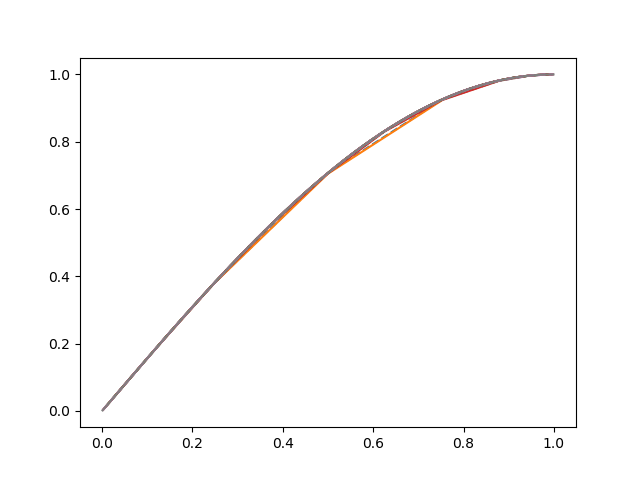
\includegraphics[width=\linewidth]{1.png}
		\caption{$\Delta t = \frac{h^2}{2a}(0.001)$.}
	\end{subfigure}
	\begin{subfigure}[b]{0.4\linewidth}
		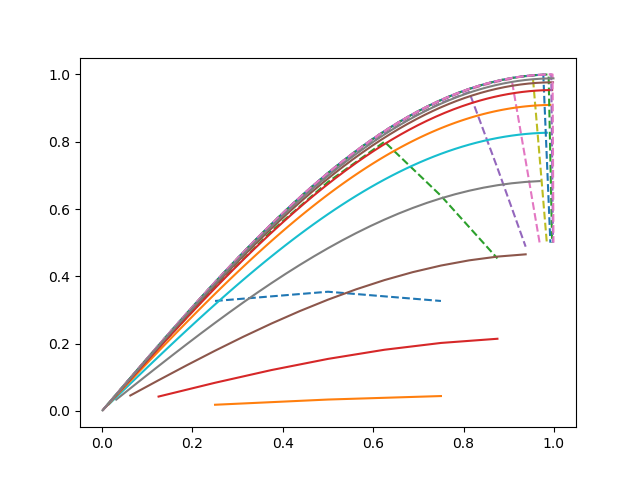
\includegraphics[width=\linewidth]{2.png}
		\caption{$\Delta t = \frac{h^2}{2a} (0.999)$.}
	\end{subfigure}
	\caption{the dashed lines are the approximations. It is clear that is is closer to the analytical solution as $h$ tend to $\frac{1}{1024}$.}
	\label{fig:cmp1}
\end{figure}
\paragraph{}We see that the solution is closer as $h$ is smaller, if whe compare both solutions only on $h = \frac{1}{1024}$.
\begin{figure}[h!]
	\centering
	\begin{subfigure}[b]{0.4\linewidth}
		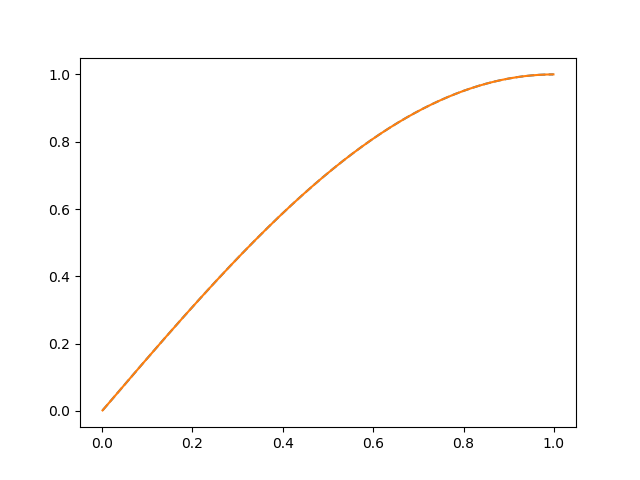
\includegraphics[width=\linewidth]{3.png}
		\caption{$\Delta t = \frac{h^2}{2a}(0.001)$.}
	\end{subfigure}
	\begin{subfigure}[b]{0.4\linewidth}
		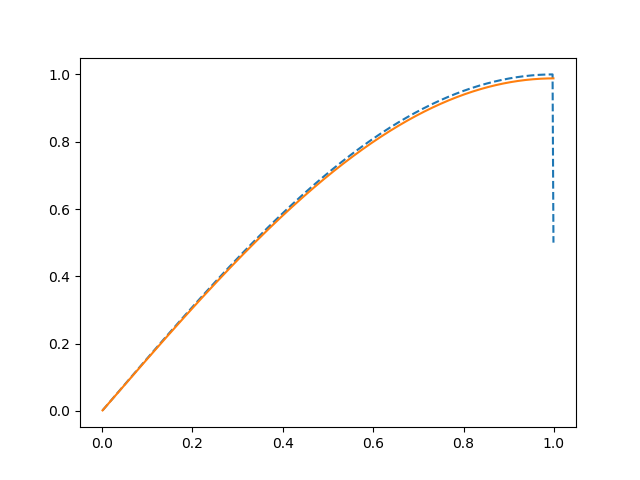
\includegraphics[width=\linewidth]{4.png}
		\caption{$\Delta t = \frac{h^2}{2a} (0.999)$.}
	\end{subfigure}
	\caption{the dashed lines are the approximations.}
	\label{fig:cmp2}
\end{figure}
\paragraph{}A closer zoom on a gives us a clear answer of which parameter is better.
\newpage
\begin{figure}[h!]
	\centering
	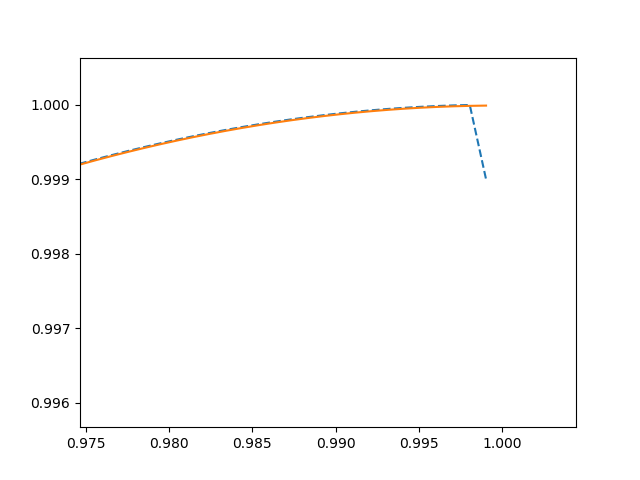
\includegraphics[width=0.5\linewidth]{5.png}
\end{figure}
We can conclude that the best parameter to choose on this problem as $h$ approaches zero is $\Delta t = \frac{h^2}{2a}(0.001)$. But at this point we can also see that the error relies on the last points of the estimation, this is happening because as x approaches to $1$, the formula changes, and the initial solution is given by the formula $e^{-\pi^2 \frac{t}{4}}$.
\paragraph{3} Please load the CVS attached to the midterm and perform constant, linear, cuadratic and cubic regression ¿What regression fits the bests?
\paragraph{Solution.} After performing each of the regressions we get\footnote{The data of the solution is on the excel file}:
\begin{figure}[h!]
	\centering
	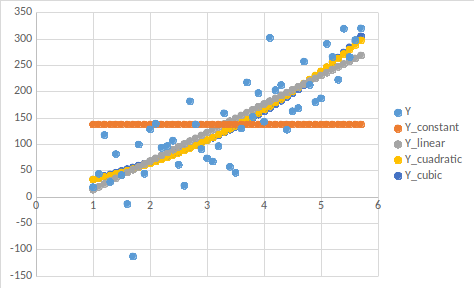
\includegraphics[width=0.5\linewidth]{6.png}
\end{figure}
\paragraph{}We clealy see that the closests approximations would be the cuadratic and the cubic form, it is expected than the cubic form will perform better, which is why we compare the absolute error on both solutions, the solution with the lowest error will be a better approximation.\newpage
\begin{figure}[h!]
	\centering
	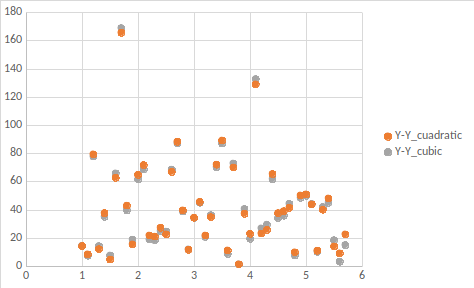
\includegraphics[width=0.5\linewidth]{7.png}
\end{figure}
\paragraph{} Both of solutions seem to be closer to the initial points, so we use the average to check in general wich solution is closer, for the cuadratic aproximation we get $\approx 41.44$, on the cubic form we get $\approx 40.98$. The cubic form in general is more precise
\end{document}